\documentclass{article}
\usepackage{booktabs}
\usepackage{graphicx}
\makeatletter
\setlength{\@fptop}{0pt}
\makeatother

\title{Biol 461 Winter 2021 TA Section 02/19/21}
\author{}
\date{}

\begin{document}

\maketitle
\noindent Figures taken from:
Keller, Andreas, Hanyi Zhuang, Qiuyi Chi, Leslie B. Vosshall, and Hiroaki Matsunami. “Genetic Variation in a Human Odorant Receptor Alters Odour Perception.” Nature 449, no. 7161 (2007): 468–72. \\https://doi.org/10.1038/nature06162.
\\
\\
Androstone is an odorous steroid that is known to smell very different to different people. Scientists wanted to see if this difference could be due to differences in the odorant receptor(s) that is (are) sensitive to Androstone.

\section{}
First the odorant receptor(s) sensitive to Androstone had to be identified. Scientists cloned 335 human odorant receptors (ORs) and expressed them in cells in culture (such that there was a unique culture for each OR; each culture only expressed one OR). They performed a functional florescence assay to see which ORs were activated by Androstone. These results are shown (for 56 of the receptors) in Part A of the below figure:

\begin{figure}[h]
\hspace*{-3cm} 
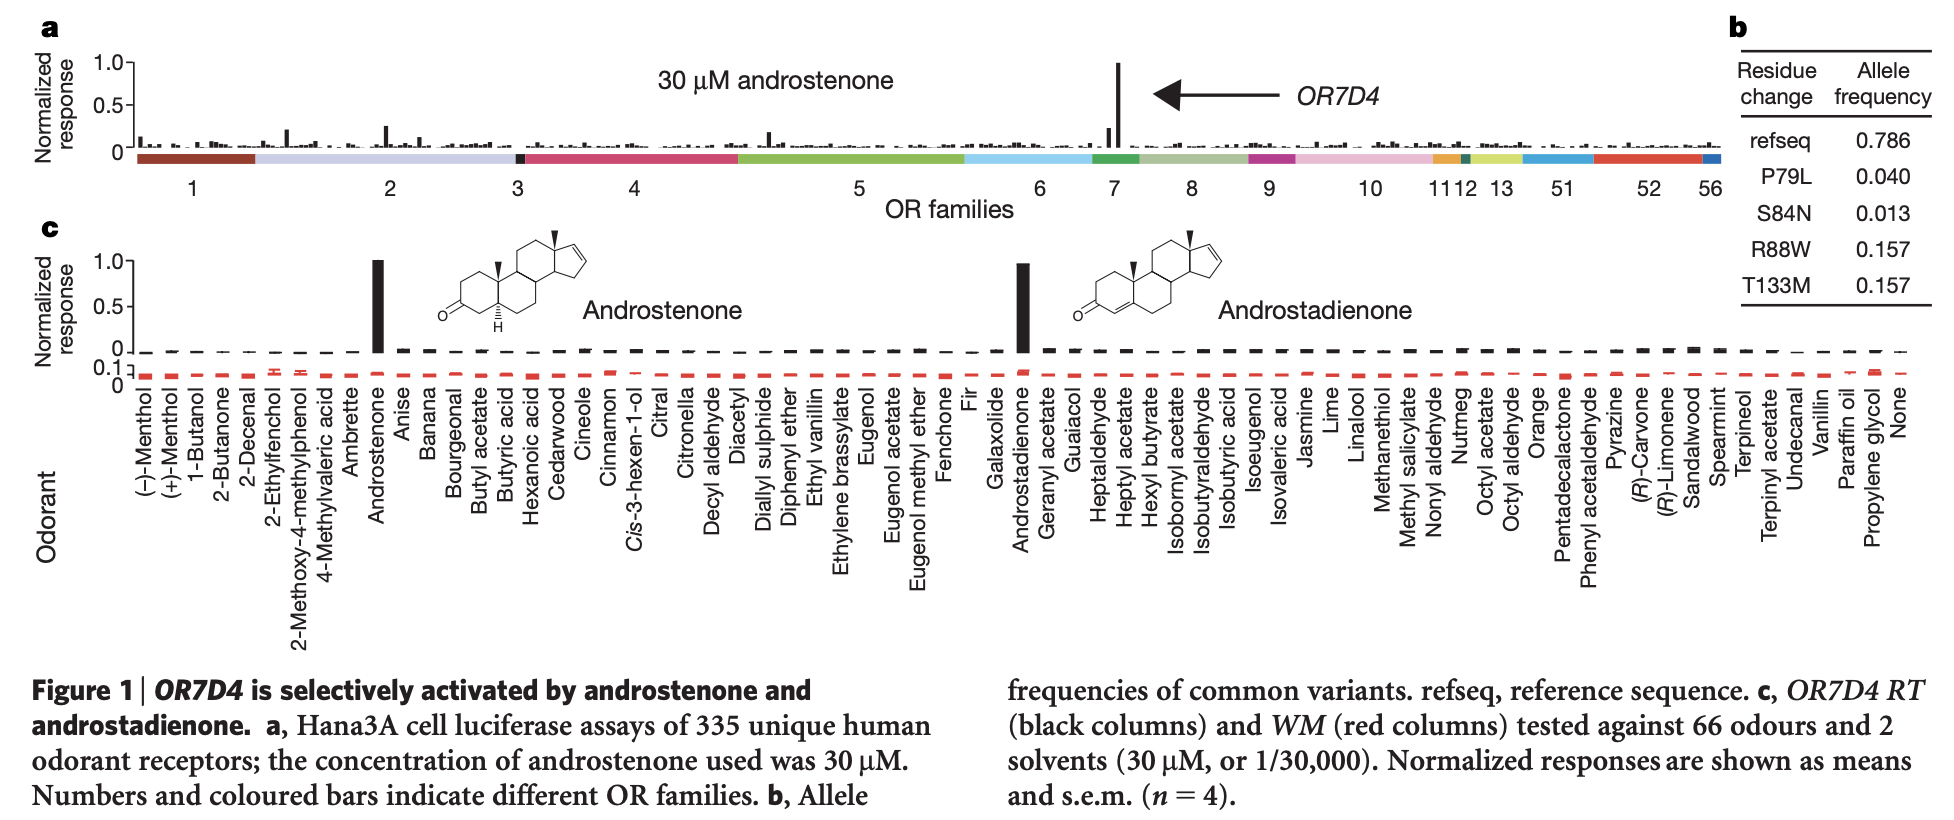
\includegraphics[scale =.5]{1.1}\\
\end{figure}

\noindent \textbf{QUESTION 1:} Which OR had the strongest response to Androstenone?\\
\\
\\
\section{}
Scientists looked in genomic databases to identify the most common non-synonymous polymorphisms found in humans in the gene coding for this OR. The four most common non-synonymous SNPs found are shown in part b of figure 1 above (refseq is the referece sequence).\\\\
\textbf{QUESTION 2a:} What is a non-synonymous polymorphism?\\\\
\textbf{QUESTION 2b:} What were the two most common non-synonymous SNPs? What are their frequencies? What does this suggest about these SNPs?\\
\\
\\
\section{}
These two SNPs were found to be in complete linkage disequilibrium and result in two amino acid changes in the OR. Scientists expressed the OR with those amino acid changes in a cell line and compared the responses of cells expressing the reference sequence OR (termed the RT OR) vs cells expressing this different version (termed the WM OR) to 66 different odours and the two solvents the odors were dissolved in. The data from these functional assays is showin in part c of figure 1 above. \\\\
\textbf{QUESTION 3a:} What does it mean that these SNPs are in complete linkage disequilibrium?\\\\
\textbf{QUESTION 3b:} Why did the scientists test to see if the ORs responded to the solvents?\\\\
\textbf{QUESTION 3c:} What odors/solvents are the RT ORs most sensitive to?\\\\
\textbf{QUESTION 3d:} How do the responses of the two ORs differ?\\\\

\section{}
The scientists investigated the structural differences between the RT OR and the WM OR and calculated dose response curves and EC$_50$s for each in relation to Androstenone and Androstadienone. We are going to skip that part for now. \\
\\
Next scientists wanted to see if people with one (or two) WM allele(s) perceived smells differently (especially the smells of Androstenone and Androstadienone). Genotyped volunteers were asked to smell the 66 different odors (and the 2 solvents) at two concentrations and asked to rank the intensity and pleasantness of each smell. The data from these experiments are shown in the two images below:\break

\renewcommand{\thefigure}{3a}
\begin{figure}[h]
\hspace*{-3.5cm} 
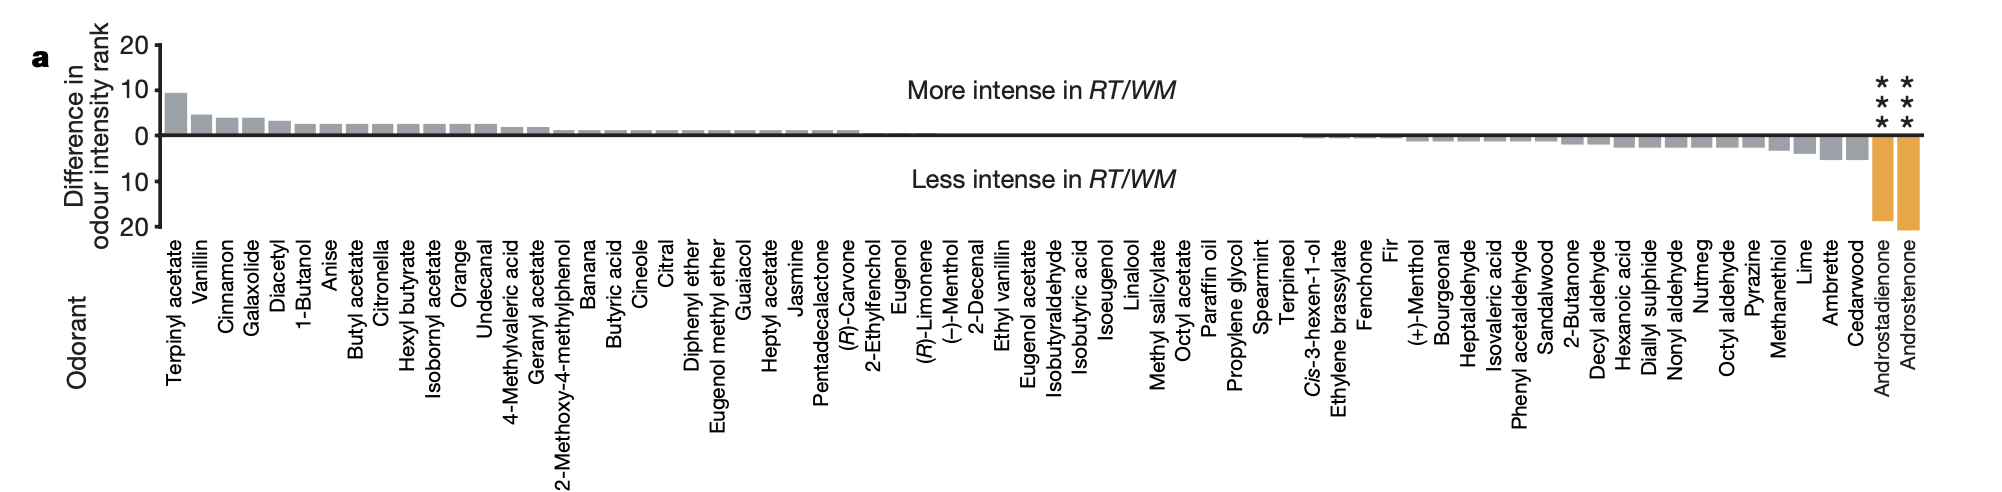
\includegraphics[scale =.55]{3}\\
\caption{OR7D4 variation affects androstenone and androstadienone intensity perception. a, Differences in median odour intensity ranking of 66 odours and 2 solvents between OR7D4 RT/WM and RT/RT groups. Data for two different odour concentrations were pooled. }
\renewcommand{\thefigure}{4a}
\hspace*{-3.5cm} 
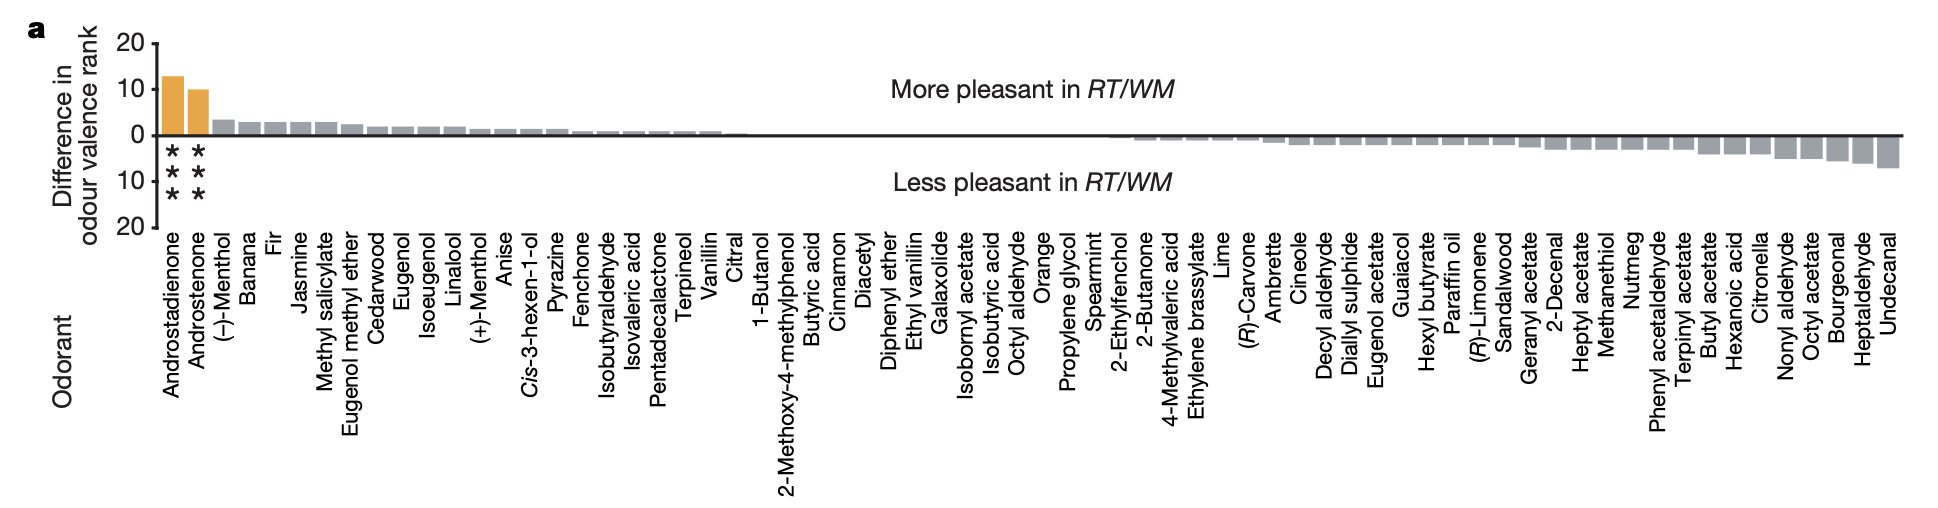
\includegraphics[scale =.55]{5}\\
\caption{Differences in median odour valence ranking for the same odours and genotypes as in Fig. 3a.}
\end{figure}
\vspace{35mm}

\noindent \textbf{QUESTION 4a:} What is the Y axis in these figures?\\
\\
\textbf{QUESTION 4b:} What compounds yielded significant differences between volunteers with RT/RT genotypes vs volunteers with RT/WM genotypes in each figure? Which population found these compounds more intense? Which population found these compound more pleasant?\\
\\
\textbf{QUESTION 4c:} What do these results suggest about the mechanism underlying differences in the perception of Androstone?
\end{document}
